% Created by tikzDevice version 0.12.3.1 on 2022-07-29 15:54:15
% !TEX encoding = UTF-8 Unicode
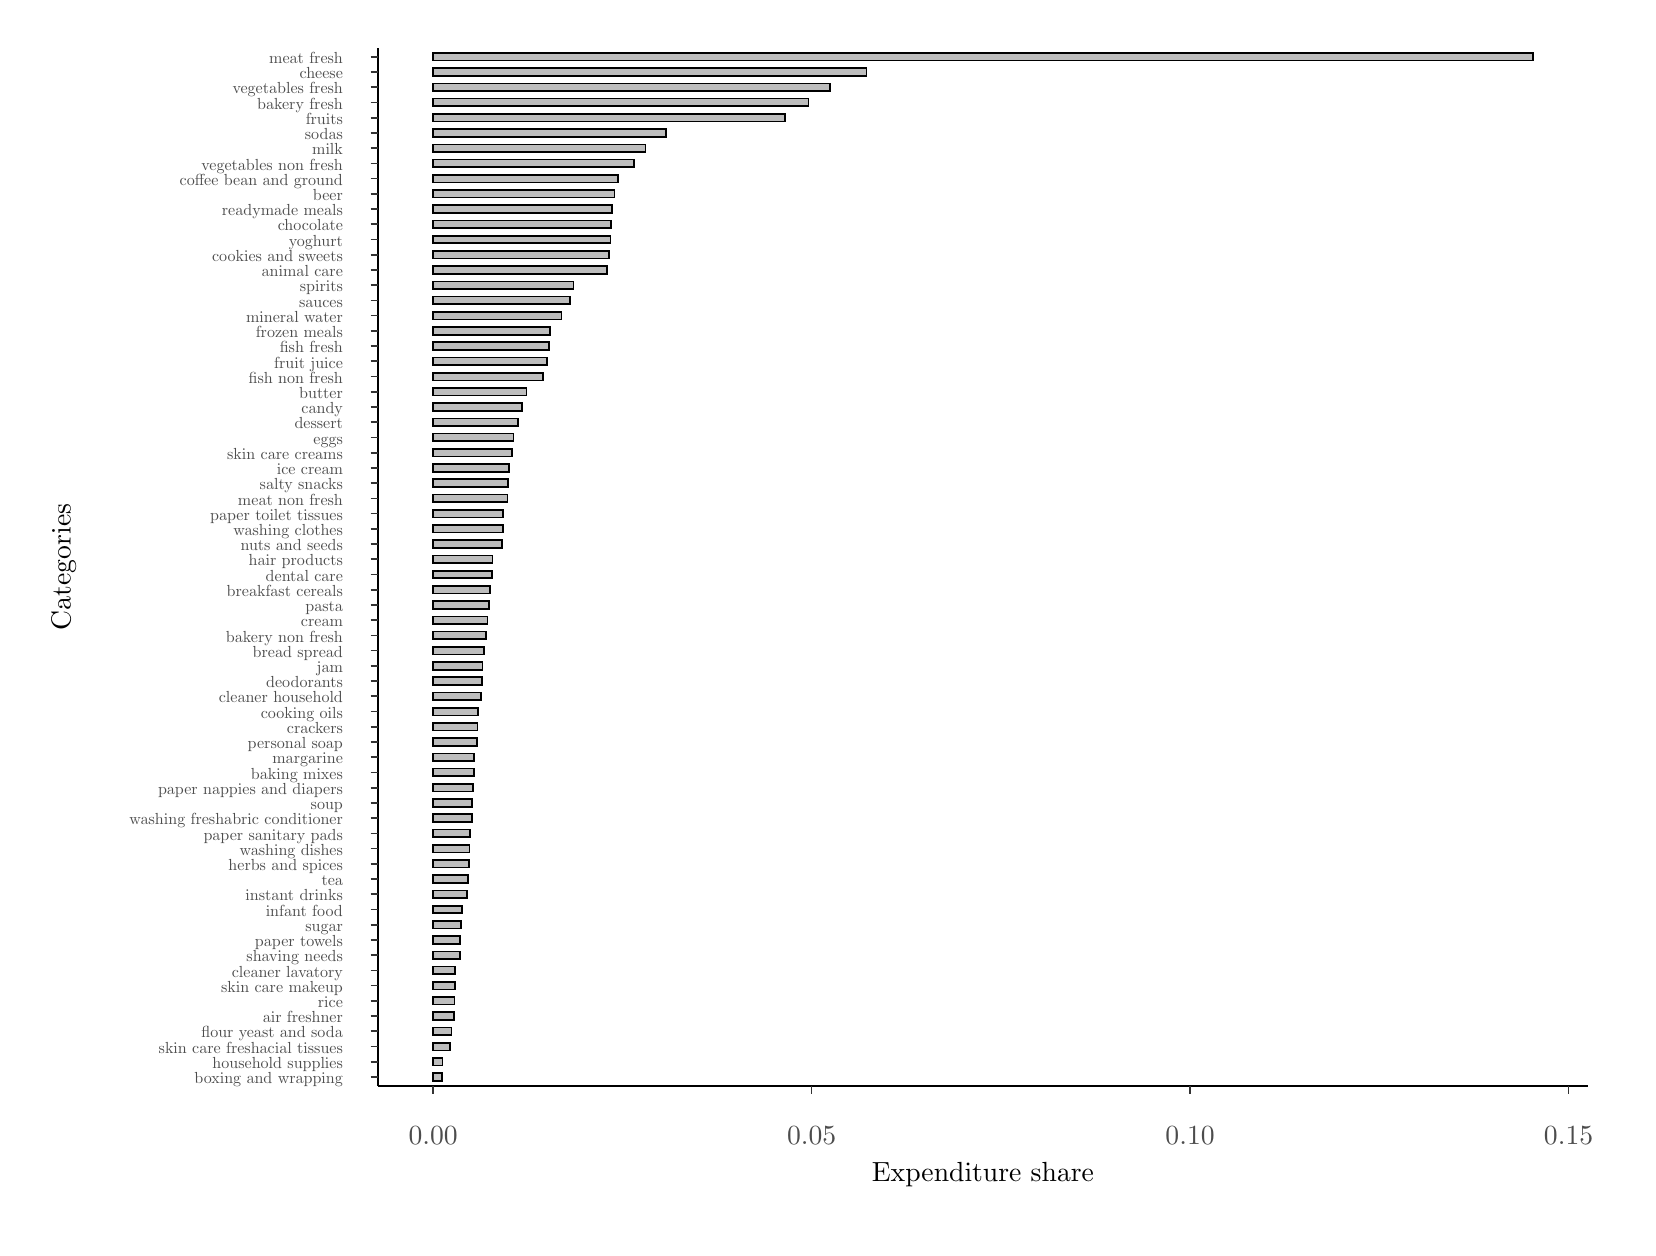
\begin{tikzpicture}[x=1pt,y=1pt]
\definecolor{fillColor}{RGB}{255,255,255}
\path[use as bounding box,fill=fillColor,fill opacity=0.00] (0,0) rectangle (578.16,433.62);
\begin{scope}
\path[clip] (  0.00,  0.00) rectangle (578.16,433.62);
\definecolor{drawColor}{RGB}{255,255,255}
\definecolor{fillColor}{RGB}{255,255,255}

\path[draw=drawColor,line width= 0.6pt,line join=round,line cap=round,fill=fillColor] (  0.00,  0.00) rectangle (578.16,433.62);
\end{scope}
\begin{scope}
\path[clip] (126.66, 51.15) rectangle (563.71,426.39);
\definecolor{drawColor}{RGB}{255,255,255}

\path[draw=drawColor,line width= 0.3pt,line join=round] (214.90, 51.15) --
	(214.90,426.39);

\path[draw=drawColor,line width= 0.3pt,line join=round] (351.66, 51.15) --
	(351.66,426.39);

\path[draw=drawColor,line width= 0.3pt,line join=round] (488.43, 51.15) --
	(488.43,426.39);
\definecolor{drawColor}{RGB}{0,0,0}
\definecolor{fillColor}{gray}{0.74}

\path[draw=drawColor,line width= 0.6pt,line cap=rect,fill=fillColor] (146.52, 75.09) rectangle (154.04, 77.84);

\path[draw=drawColor,line width= 0.6pt,line cap=rect,fill=fillColor] (146.52,344.69) rectangle (209.42,347.44);

\path[draw=drawColor,line width= 0.6pt,line cap=rect,fill=fillColor] (146.52,405.21) rectangle (282.09,407.96);

\path[draw=drawColor,line width= 0.6pt,line cap=rect,fill=fillColor] (146.52,212.64) rectangle (165.70,215.39);

\path[draw=drawColor,line width= 0.6pt,line cap=rect,fill=fillColor] (146.52,163.12) rectangle (161.16,165.87);

\path[draw=drawColor,line width= 0.6pt,line cap=rect,fill=fillColor] (146.52,372.20) rectangle (212.09,374.95);

\path[draw=drawColor,line width= 0.6pt,line cap=rect,fill=fillColor] (146.52, 53.08) rectangle (149.82, 55.83);

\path[draw=drawColor,line width= 0.6pt,line cap=rect,fill=fillColor] (146.52,207.14) rectangle (164.95,209.89);

\path[draw=drawColor,line width= 0.6pt,line cap=rect,fill=fillColor] (146.52,229.14) rectangle (167.02,231.90);

\path[draw=drawColor,line width= 0.6pt,line cap=rect,fill=fillColor] (146.52,300.67) rectangle (180.26,303.42);

\path[draw=drawColor,line width= 0.6pt,line cap=rect,fill=fillColor] (146.52,295.17) rectangle (178.63,297.92);

\path[draw=drawColor,line width= 0.6pt,line cap=rect,fill=fillColor] (146.52,416.21) rectangle (303.15,418.97);

\path[draw=drawColor,line width= 0.6pt,line cap=rect,fill=fillColor] (146.52,361.19) rectangle (210.69,363.94);

\path[draw=drawColor,line width= 0.6pt,line cap=rect,fill=fillColor] (146.52,190.63) rectangle (163.75,193.38);

\path[draw=drawColor,line width= 0.6pt,line cap=rect,fill=fillColor] (146.52, 91.59) rectangle (154.47, 94.34);

\path[draw=drawColor,line width= 0.6pt,line cap=rect,fill=fillColor] (146.52,377.70) rectangle (213.32,380.45);

\path[draw=drawColor,line width= 0.6pt,line cap=rect,fill=fillColor] (146.52,350.19) rectangle (210.12,352.94);

\path[draw=drawColor,line width= 0.6pt,line cap=rect,fill=fillColor] (146.52,185.13) rectangle (162.63,187.88);

\path[draw=drawColor,line width= 0.6pt,line cap=rect,fill=fillColor] (146.52,179.63) rectangle (162.55,182.38);

\path[draw=drawColor,line width= 0.6pt,line cap=rect,fill=fillColor] (146.52,218.14) rectangle (166.12,220.89);

\path[draw=drawColor,line width= 0.6pt,line cap=rect,fill=fillColor] (146.52,234.65) rectangle (167.81,237.40);

\path[draw=drawColor,line width= 0.6pt,line cap=rect,fill=fillColor] (146.52,196.13) rectangle (164.12,198.88);

\path[draw=drawColor,line width= 0.6pt,line cap=rect,fill=fillColor] (146.52,289.67) rectangle (177.15,292.42);

\path[draw=drawColor,line width= 0.6pt,line cap=rect,fill=fillColor] (146.52,284.17) rectangle (175.55,286.92);

\path[draw=drawColor,line width= 0.6pt,line cap=rect,fill=fillColor] (146.52,317.18) rectangle (188.43,319.93);

\path[draw=drawColor,line width= 0.6pt,line cap=rect,fill=fillColor] (146.52,306.17) rectangle (186.26,308.92);

\path[draw=drawColor,line width= 0.6pt,line cap=rect,fill=fillColor] (146.52, 69.59) rectangle (153.09, 72.34);

\path[draw=drawColor,line width= 0.6pt,line cap=rect,fill=fillColor] (146.52,322.68) rectangle (188.77,325.43);

\path[draw=drawColor,line width= 0.6pt,line cap=rect,fill=fillColor] (146.52,311.68) rectangle (187.64,314.43);

\path[draw=drawColor,line width= 0.6pt,line cap=rect,fill=fillColor] (146.52,399.71) rectangle (273.77,402.46);

\path[draw=drawColor,line width= 0.6pt,line cap=rect,fill=fillColor] (146.52,240.15) rectangle (167.98,242.90);

\path[draw=drawColor,line width= 0.6pt,line cap=rect,fill=fillColor] (146.52,130.11) rectangle (159.57,132.86);

\path[draw=drawColor,line width= 0.6pt,line cap=rect,fill=fillColor] (146.52, 58.58) rectangle (149.85, 61.33);

\path[draw=drawColor,line width= 0.6pt,line cap=rect,fill=fillColor] (146.52,273.16) rectangle (173.92,275.91);

\path[draw=drawColor,line width= 0.6pt,line cap=rect,fill=fillColor] (146.52,113.60) rectangle (156.88,116.35);

\path[draw=drawColor,line width= 0.6pt,line cap=rect,fill=fillColor] (146.52,119.10) rectangle (158.85,121.85);

\path[draw=drawColor,line width= 0.6pt,line cap=rect,fill=fillColor] (146.52,201.63) rectangle (164.37,204.39);

\path[draw=drawColor,line width= 0.6pt,line cap=rect,fill=fillColor] (146.52,168.62) rectangle (161.36,171.37);

\path[draw=drawColor,line width= 0.6pt,line cap=rect,fill=fillColor] (146.52,421.72) rectangle (543.84,424.47);

\path[draw=drawColor,line width= 0.6pt,line cap=rect,fill=fillColor] (146.52,262.16) rectangle (173.44,264.91);

\path[draw=drawColor,line width= 0.6pt,line cap=rect,fill=fillColor] (146.52,388.70) rectangle (223.21,391.46);

\path[draw=drawColor,line width= 0.6pt,line cap=rect,fill=fillColor] (146.52,328.18) rectangle (192.94,330.93);

\path[draw=drawColor,line width= 0.6pt,line cap=rect,fill=fillColor] (146.52,245.65) rectangle (171.39,248.40);

\path[draw=drawColor,line width= 0.6pt,line cap=rect,fill=fillColor] (146.52,157.62) rectangle (160.85,160.37);

\path[draw=drawColor,line width= 0.6pt,line cap=rect,fill=fillColor] (146.52,141.11) rectangle (159.86,143.86);

\path[draw=drawColor,line width= 0.6pt,line cap=rect,fill=fillColor] (146.52,256.65) rectangle (171.87,259.41);

\path[draw=drawColor,line width= 0.6pt,line cap=rect,fill=fillColor] (146.52,102.60) rectangle (156.27,105.35);

\path[draw=drawColor,line width= 0.6pt,line cap=rect,fill=fillColor] (146.52,223.64) rectangle (166.60,226.39);

\path[draw=drawColor,line width= 0.6pt,line cap=rect,fill=fillColor] (146.52,174.12) rectangle (162.27,176.88);

\path[draw=drawColor,line width= 0.6pt,line cap=rect,fill=fillColor] (146.52,366.70) rectangle (211.04,369.45);

\path[draw=drawColor,line width= 0.6pt,line cap=rect,fill=fillColor] (146.52, 80.59) rectangle (154.17, 83.34);

\path[draw=drawColor,line width= 0.6pt,line cap=rect,fill=fillColor] (146.52,267.66) rectangle (173.62,270.41);

\path[draw=drawColor,line width= 0.6pt,line cap=rect,fill=fillColor] (146.52,333.68) rectangle (196.02,336.43);

\path[draw=drawColor,line width= 0.6pt,line cap=rect,fill=fillColor] (146.52, 97.10) rectangle (156.12, 99.85);

\path[draw=drawColor,line width= 0.6pt,line cap=rect,fill=fillColor] (146.52,278.66) rectangle (174.90,281.41);

\path[draw=drawColor,line width= 0.6pt,line cap=rect,fill=fillColor] (146.52, 64.08) rectangle (152.64, 66.83);

\path[draw=drawColor,line width= 0.6pt,line cap=rect,fill=fillColor] (146.52, 86.09) rectangle (154.43, 88.84);

\path[draw=drawColor,line width= 0.6pt,line cap=rect,fill=fillColor] (146.52,394.21) rectangle (230.69,396.96);

\path[draw=drawColor,line width= 0.6pt,line cap=rect,fill=fillColor] (146.52,152.12) rectangle (160.67,154.87);

\path[draw=drawColor,line width= 0.6pt,line cap=rect,fill=fillColor] (146.52,339.19) rectangle (197.27,341.94);

\path[draw=drawColor,line width= 0.6pt,line cap=rect,fill=fillColor] (146.52,108.10) rectangle (156.59,110.85);

\path[draw=drawColor,line width= 0.6pt,line cap=rect,fill=fillColor] (146.52,124.61) rectangle (159.13,127.36);

\path[draw=drawColor,line width= 0.6pt,line cap=rect,fill=fillColor] (146.52,410.71) rectangle (289.84,413.46);

\path[draw=drawColor,line width= 0.6pt,line cap=rect,fill=fillColor] (146.52,383.20) rectangle (219.04,385.95);

\path[draw=drawColor,line width= 0.6pt,line cap=rect,fill=fillColor] (146.52,251.15) rectangle (171.73,253.90);

\path[draw=drawColor,line width= 0.6pt,line cap=rect,fill=fillColor] (146.52,135.61) rectangle (159.71,138.36);

\path[draw=drawColor,line width= 0.6pt,line cap=rect,fill=fillColor] (146.52,146.61) rectangle (160.56,149.37);

\path[draw=drawColor,line width= 0.6pt,line cap=rect,fill=fillColor] (146.52,355.69) rectangle (210.60,358.44);
\end{scope}
\begin{scope}
\path[clip] (  0.00,  0.00) rectangle (578.16,433.62);
\definecolor{drawColor}{RGB}{0,0,0}

\path[draw=drawColor,line width= 0.6pt,line join=round] (126.66, 51.15) --
	(126.66,426.39);
\end{scope}
\begin{scope}
\path[clip] (  0.00,  0.00) rectangle (578.16,433.62);
\definecolor{drawColor}{gray}{0.30}

\node[text=drawColor,anchor=base east,inner sep=0pt, outer sep=0pt, scale=  0.58] at (113.91, 52.04) {boxing and wrapping};

\node[text=drawColor,anchor=base east,inner sep=0pt, outer sep=0pt, scale=  0.58] at (113.91, 57.55) {household supplies};

\node[text=drawColor,anchor=base east,inner sep=0pt, outer sep=0pt, scale=  0.58] at (113.91, 63.05) {skin care freshacial tissues};

\node[text=drawColor,anchor=base east,inner sep=0pt, outer sep=0pt, scale=  0.58] at (113.91, 68.55) {flour yeast and soda};

\node[text=drawColor,anchor=base east,inner sep=0pt, outer sep=0pt, scale=  0.58] at (113.91, 74.05) {air freshner};

\node[text=drawColor,anchor=base east,inner sep=0pt, outer sep=0pt, scale=  0.58] at (113.91, 79.55) {rice};

\node[text=drawColor,anchor=base east,inner sep=0pt, outer sep=0pt, scale=  0.58] at (113.91, 85.06) {skin care  makeup};

\node[text=drawColor,anchor=base east,inner sep=0pt, outer sep=0pt, scale=  0.58] at (113.91, 90.56) {cleaner  lavatory};

\node[text=drawColor,anchor=base east,inner sep=0pt, outer sep=0pt, scale=  0.58] at (113.91, 96.06) {shaving needs};

\node[text=drawColor,anchor=base east,inner sep=0pt, outer sep=0pt, scale=  0.58] at (113.91,101.56) {paper  towels};

\node[text=drawColor,anchor=base east,inner sep=0pt, outer sep=0pt, scale=  0.58] at (113.91,107.06) {sugar};

\node[text=drawColor,anchor=base east,inner sep=0pt, outer sep=0pt, scale=  0.58] at (113.91,112.57) {infant food};

\node[text=drawColor,anchor=base east,inner sep=0pt, outer sep=0pt, scale=  0.58] at (113.91,118.07) {instant drinks};

\node[text=drawColor,anchor=base east,inner sep=0pt, outer sep=0pt, scale=  0.58] at (113.91,123.57) {tea};

\node[text=drawColor,anchor=base east,inner sep=0pt, outer sep=0pt, scale=  0.58] at (113.91,129.07) {herbs and spices};

\node[text=drawColor,anchor=base east,inner sep=0pt, outer sep=0pt, scale=  0.58] at (113.91,134.57) {washing  dishes};

\node[text=drawColor,anchor=base east,inner sep=0pt, outer sep=0pt, scale=  0.58] at (113.91,140.08) {paper  sanitary pads};

\node[text=drawColor,anchor=base east,inner sep=0pt, outer sep=0pt, scale=  0.58] at (113.91,145.58) {washing freshabric conditioner};

\node[text=drawColor,anchor=base east,inner sep=0pt, outer sep=0pt, scale=  0.58] at (113.91,151.08) {soup};

\node[text=drawColor,anchor=base east,inner sep=0pt, outer sep=0pt, scale=  0.58] at (113.91,156.58) {paper  nappies and diapers};

\node[text=drawColor,anchor=base east,inner sep=0pt, outer sep=0pt, scale=  0.58] at (113.91,162.08) {baking mixes};

\node[text=drawColor,anchor=base east,inner sep=0pt, outer sep=0pt, scale=  0.58] at (113.91,167.59) {margarine};

\node[text=drawColor,anchor=base east,inner sep=0pt, outer sep=0pt, scale=  0.58] at (113.91,173.09) {personal soap};

\node[text=drawColor,anchor=base east,inner sep=0pt, outer sep=0pt, scale=  0.58] at (113.91,178.59) {crackers};

\node[text=drawColor,anchor=base east,inner sep=0pt, outer sep=0pt, scale=  0.58] at (113.91,184.09) {cooking oils};

\node[text=drawColor,anchor=base east,inner sep=0pt, outer sep=0pt, scale=  0.58] at (113.91,189.60) {cleaner  household};

\node[text=drawColor,anchor=base east,inner sep=0pt, outer sep=0pt, scale=  0.58] at (113.91,195.10) {deodorants};

\node[text=drawColor,anchor=base east,inner sep=0pt, outer sep=0pt, scale=  0.58] at (113.91,200.60) {jam};

\node[text=drawColor,anchor=base east,inner sep=0pt, outer sep=0pt, scale=  0.58] at (113.91,206.10) {bread spread};

\node[text=drawColor,anchor=base east,inner sep=0pt, outer sep=0pt, scale=  0.58] at (113.91,211.60) {bakery non fresh};

\node[text=drawColor,anchor=base east,inner sep=0pt, outer sep=0pt, scale=  0.58] at (113.91,217.11) {cream};

\node[text=drawColor,anchor=base east,inner sep=0pt, outer sep=0pt, scale=  0.58] at (113.91,222.61) {pasta};

\node[text=drawColor,anchor=base east,inner sep=0pt, outer sep=0pt, scale=  0.58] at (113.91,228.11) {breakfast cereals};

\node[text=drawColor,anchor=base east,inner sep=0pt, outer sep=0pt, scale=  0.58] at (113.91,233.61) {dental care};

\node[text=drawColor,anchor=base east,inner sep=0pt, outer sep=0pt, scale=  0.58] at (113.91,239.11) {hair products};

\node[text=drawColor,anchor=base east,inner sep=0pt, outer sep=0pt, scale=  0.58] at (113.91,244.62) {nuts and seeds};

\node[text=drawColor,anchor=base east,inner sep=0pt, outer sep=0pt, scale=  0.58] at (113.91,250.12) {washing  clothes};

\node[text=drawColor,anchor=base east,inner sep=0pt, outer sep=0pt, scale=  0.58] at (113.91,255.62) {paper  toilet tissues};

\node[text=drawColor,anchor=base east,inner sep=0pt, outer sep=0pt, scale=  0.58] at (113.91,261.12) {meat non fresh};

\node[text=drawColor,anchor=base east,inner sep=0pt, outer sep=0pt, scale=  0.58] at (113.91,266.62) {salty snacks};

\node[text=drawColor,anchor=base east,inner sep=0pt, outer sep=0pt, scale=  0.58] at (113.91,272.13) {ice cream};

\node[text=drawColor,anchor=base east,inner sep=0pt, outer sep=0pt, scale=  0.58] at (113.91,277.63) {skin care  creams};

\node[text=drawColor,anchor=base east,inner sep=0pt, outer sep=0pt, scale=  0.58] at (113.91,283.13) {eggs};

\node[text=drawColor,anchor=base east,inner sep=0pt, outer sep=0pt, scale=  0.58] at (113.91,288.63) {dessert};

\node[text=drawColor,anchor=base east,inner sep=0pt, outer sep=0pt, scale=  0.58] at (113.91,294.13) {candy};

\node[text=drawColor,anchor=base east,inner sep=0pt, outer sep=0pt, scale=  0.58] at (113.91,299.64) {butter};

\node[text=drawColor,anchor=base east,inner sep=0pt, outer sep=0pt, scale=  0.58] at (113.91,305.14) {fish non fresh};

\node[text=drawColor,anchor=base east,inner sep=0pt, outer sep=0pt, scale=  0.58] at (113.91,310.64) {fruit juice};

\node[text=drawColor,anchor=base east,inner sep=0pt, outer sep=0pt, scale=  0.58] at (113.91,316.14) {fish fresh};

\node[text=drawColor,anchor=base east,inner sep=0pt, outer sep=0pt, scale=  0.58] at (113.91,321.64) {frozen meals};

\node[text=drawColor,anchor=base east,inner sep=0pt, outer sep=0pt, scale=  0.58] at (113.91,327.15) {mineral water};

\node[text=drawColor,anchor=base east,inner sep=0pt, outer sep=0pt, scale=  0.58] at (113.91,332.65) {sauces};

\node[text=drawColor,anchor=base east,inner sep=0pt, outer sep=0pt, scale=  0.58] at (113.91,338.15) {spirits};

\node[text=drawColor,anchor=base east,inner sep=0pt, outer sep=0pt, scale=  0.58] at (113.91,343.65) {animal care};

\node[text=drawColor,anchor=base east,inner sep=0pt, outer sep=0pt, scale=  0.58] at (113.91,349.15) {cookies and sweets};

\node[text=drawColor,anchor=base east,inner sep=0pt, outer sep=0pt, scale=  0.58] at (113.91,354.66) {yoghurt};

\node[text=drawColor,anchor=base east,inner sep=0pt, outer sep=0pt, scale=  0.58] at (113.91,360.16) {chocolate};

\node[text=drawColor,anchor=base east,inner sep=0pt, outer sep=0pt, scale=  0.58] at (113.91,365.66) {readymade meals};

\node[text=drawColor,anchor=base east,inner sep=0pt, outer sep=0pt, scale=  0.58] at (113.91,371.16) {beer};

\node[text=drawColor,anchor=base east,inner sep=0pt, outer sep=0pt, scale=  0.58] at (113.91,376.66) {coffee  bean and ground};

\node[text=drawColor,anchor=base east,inner sep=0pt, outer sep=0pt, scale=  0.58] at (113.91,382.17) {vegetables non fresh};

\node[text=drawColor,anchor=base east,inner sep=0pt, outer sep=0pt, scale=  0.58] at (113.91,387.67) {milk};

\node[text=drawColor,anchor=base east,inner sep=0pt, outer sep=0pt, scale=  0.58] at (113.91,393.17) {sodas};

\node[text=drawColor,anchor=base east,inner sep=0pt, outer sep=0pt, scale=  0.58] at (113.91,398.67) {fruits};

\node[text=drawColor,anchor=base east,inner sep=0pt, outer sep=0pt, scale=  0.58] at (113.91,404.17) {bakery fresh};

\node[text=drawColor,anchor=base east,inner sep=0pt, outer sep=0pt, scale=  0.58] at (113.91,409.68) {vegetables fresh};

\node[text=drawColor,anchor=base east,inner sep=0pt, outer sep=0pt, scale=  0.58] at (113.91,415.18) {cheese};

\node[text=drawColor,anchor=base east,inner sep=0pt, outer sep=0pt, scale=  0.58] at (113.91,420.68) {meat fresh};
\end{scope}
\begin{scope}
\path[clip] (  0.00,  0.00) rectangle (578.16,433.62);
\definecolor{drawColor}{gray}{0.20}

\path[draw=drawColor,line width= 0.6pt,line join=round] (123.91, 54.45) --
	(126.66, 54.45);

\path[draw=drawColor,line width= 0.6pt,line join=round] (123.91, 59.96) --
	(126.66, 59.96);

\path[draw=drawColor,line width= 0.6pt,line join=round] (123.91, 65.46) --
	(126.66, 65.46);

\path[draw=drawColor,line width= 0.6pt,line join=round] (123.91, 70.96) --
	(126.66, 70.96);

\path[draw=drawColor,line width= 0.6pt,line join=round] (123.91, 76.46) --
	(126.66, 76.46);

\path[draw=drawColor,line width= 0.6pt,line join=round] (123.91, 81.97) --
	(126.66, 81.97);

\path[draw=drawColor,line width= 0.6pt,line join=round] (123.91, 87.47) --
	(126.66, 87.47);

\path[draw=drawColor,line width= 0.6pt,line join=round] (123.91, 92.97) --
	(126.66, 92.97);

\path[draw=drawColor,line width= 0.6pt,line join=round] (123.91, 98.47) --
	(126.66, 98.47);

\path[draw=drawColor,line width= 0.6pt,line join=round] (123.91,103.97) --
	(126.66,103.97);

\path[draw=drawColor,line width= 0.6pt,line join=round] (123.91,109.48) --
	(126.66,109.48);

\path[draw=drawColor,line width= 0.6pt,line join=round] (123.91,114.98) --
	(126.66,114.98);

\path[draw=drawColor,line width= 0.6pt,line join=round] (123.91,120.48) --
	(126.66,120.48);

\path[draw=drawColor,line width= 0.6pt,line join=round] (123.91,125.98) --
	(126.66,125.98);

\path[draw=drawColor,line width= 0.6pt,line join=round] (123.91,131.48) --
	(126.66,131.48);

\path[draw=drawColor,line width= 0.6pt,line join=round] (123.91,136.99) --
	(126.66,136.99);

\path[draw=drawColor,line width= 0.6pt,line join=round] (123.91,142.49) --
	(126.66,142.49);

\path[draw=drawColor,line width= 0.6pt,line join=round] (123.91,147.99) --
	(126.66,147.99);

\path[draw=drawColor,line width= 0.6pt,line join=round] (123.91,153.49) --
	(126.66,153.49);

\path[draw=drawColor,line width= 0.6pt,line join=round] (123.91,158.99) --
	(126.66,158.99);

\path[draw=drawColor,line width= 0.6pt,line join=round] (123.91,164.50) --
	(126.66,164.50);

\path[draw=drawColor,line width= 0.6pt,line join=round] (123.91,170.00) --
	(126.66,170.00);

\path[draw=drawColor,line width= 0.6pt,line join=round] (123.91,175.50) --
	(126.66,175.50);

\path[draw=drawColor,line width= 0.6pt,line join=round] (123.91,181.00) --
	(126.66,181.00);

\path[draw=drawColor,line width= 0.6pt,line join=round] (123.91,186.50) --
	(126.66,186.50);

\path[draw=drawColor,line width= 0.6pt,line join=round] (123.91,192.01) --
	(126.66,192.01);

\path[draw=drawColor,line width= 0.6pt,line join=round] (123.91,197.51) --
	(126.66,197.51);

\path[draw=drawColor,line width= 0.6pt,line join=round] (123.91,203.01) --
	(126.66,203.01);

\path[draw=drawColor,line width= 0.6pt,line join=round] (123.91,208.51) --
	(126.66,208.51);

\path[draw=drawColor,line width= 0.6pt,line join=round] (123.91,214.01) --
	(126.66,214.01);

\path[draw=drawColor,line width= 0.6pt,line join=round] (123.91,219.52) --
	(126.66,219.52);

\path[draw=drawColor,line width= 0.6pt,line join=round] (123.91,225.02) --
	(126.66,225.02);

\path[draw=drawColor,line width= 0.6pt,line join=round] (123.91,230.52) --
	(126.66,230.52);

\path[draw=drawColor,line width= 0.6pt,line join=round] (123.91,236.02) --
	(126.66,236.02);

\path[draw=drawColor,line width= 0.6pt,line join=round] (123.91,241.52) --
	(126.66,241.52);

\path[draw=drawColor,line width= 0.6pt,line join=round] (123.91,247.03) --
	(126.66,247.03);

\path[draw=drawColor,line width= 0.6pt,line join=round] (123.91,252.53) --
	(126.66,252.53);

\path[draw=drawColor,line width= 0.6pt,line join=round] (123.91,258.03) --
	(126.66,258.03);

\path[draw=drawColor,line width= 0.6pt,line join=round] (123.91,263.53) --
	(126.66,263.53);

\path[draw=drawColor,line width= 0.6pt,line join=round] (123.91,269.03) --
	(126.66,269.03);

\path[draw=drawColor,line width= 0.6pt,line join=round] (123.91,274.54) --
	(126.66,274.54);

\path[draw=drawColor,line width= 0.6pt,line join=round] (123.91,280.04) --
	(126.66,280.04);

\path[draw=drawColor,line width= 0.6pt,line join=round] (123.91,285.54) --
	(126.66,285.54);

\path[draw=drawColor,line width= 0.6pt,line join=round] (123.91,291.04) --
	(126.66,291.04);

\path[draw=drawColor,line width= 0.6pt,line join=round] (123.91,296.54) --
	(126.66,296.54);

\path[draw=drawColor,line width= 0.6pt,line join=round] (123.91,302.05) --
	(126.66,302.05);

\path[draw=drawColor,line width= 0.6pt,line join=round] (123.91,307.55) --
	(126.66,307.55);

\path[draw=drawColor,line width= 0.6pt,line join=round] (123.91,313.05) --
	(126.66,313.05);

\path[draw=drawColor,line width= 0.6pt,line join=round] (123.91,318.55) --
	(126.66,318.55);

\path[draw=drawColor,line width= 0.6pt,line join=round] (123.91,324.05) --
	(126.66,324.05);

\path[draw=drawColor,line width= 0.6pt,line join=round] (123.91,329.56) --
	(126.66,329.56);

\path[draw=drawColor,line width= 0.6pt,line join=round] (123.91,335.06) --
	(126.66,335.06);

\path[draw=drawColor,line width= 0.6pt,line join=round] (123.91,340.56) --
	(126.66,340.56);

\path[draw=drawColor,line width= 0.6pt,line join=round] (123.91,346.06) --
	(126.66,346.06);

\path[draw=drawColor,line width= 0.6pt,line join=round] (123.91,351.57) --
	(126.66,351.57);

\path[draw=drawColor,line width= 0.6pt,line join=round] (123.91,357.07) --
	(126.66,357.07);

\path[draw=drawColor,line width= 0.6pt,line join=round] (123.91,362.57) --
	(126.66,362.57);

\path[draw=drawColor,line width= 0.6pt,line join=round] (123.91,368.07) --
	(126.66,368.07);

\path[draw=drawColor,line width= 0.6pt,line join=round] (123.91,373.57) --
	(126.66,373.57);

\path[draw=drawColor,line width= 0.6pt,line join=round] (123.91,379.08) --
	(126.66,379.08);

\path[draw=drawColor,line width= 0.6pt,line join=round] (123.91,384.58) --
	(126.66,384.58);

\path[draw=drawColor,line width= 0.6pt,line join=round] (123.91,390.08) --
	(126.66,390.08);

\path[draw=drawColor,line width= 0.6pt,line join=round] (123.91,395.58) --
	(126.66,395.58);

\path[draw=drawColor,line width= 0.6pt,line join=round] (123.91,401.08) --
	(126.66,401.08);

\path[draw=drawColor,line width= 0.6pt,line join=round] (123.91,406.59) --
	(126.66,406.59);

\path[draw=drawColor,line width= 0.6pt,line join=round] (123.91,412.09) --
	(126.66,412.09);

\path[draw=drawColor,line width= 0.6pt,line join=round] (123.91,417.59) --
	(126.66,417.59);

\path[draw=drawColor,line width= 0.6pt,line join=round] (123.91,423.09) --
	(126.66,423.09);
\end{scope}
\begin{scope}
\path[clip] (  0.00,  0.00) rectangle (578.16,433.62);
\definecolor{drawColor}{RGB}{0,0,0}

\path[draw=drawColor,line width= 0.6pt,line join=round] (126.66, 51.15) --
	(563.71, 51.15);
\end{scope}
\begin{scope}
\path[clip] (  0.00,  0.00) rectangle (578.16,433.62);
\definecolor{drawColor}{gray}{0.20}

\path[draw=drawColor,line width= 0.6pt,line join=round] (146.52, 48.40) --
	(146.52, 51.15);

\path[draw=drawColor,line width= 0.6pt,line join=round] (283.28, 48.40) --
	(283.28, 51.15);

\path[draw=drawColor,line width= 0.6pt,line join=round] (420.04, 48.40) --
	(420.04, 51.15);

\path[draw=drawColor,line width= 0.6pt,line join=round] (556.81, 48.40) --
	(556.81, 51.15);
\end{scope}
\begin{scope}
\path[clip] (  0.00,  0.00) rectangle (578.16,433.62);
\definecolor{drawColor}{gray}{0.30}

\node[text=drawColor,anchor=base,inner sep=0pt, outer sep=0pt, scale=  1.00] at (146.52, 30.14) {0.00};

\node[text=drawColor,anchor=base,inner sep=0pt, outer sep=0pt, scale=  1.00] at (283.28, 30.14) {0.05};

\node[text=drawColor,anchor=base,inner sep=0pt, outer sep=0pt, scale=  1.00] at (420.04, 30.14) {0.10};

\node[text=drawColor,anchor=base,inner sep=0pt, outer sep=0pt, scale=  1.00] at (556.81, 30.14) {0.15};
\end{scope}
\begin{scope}
\path[clip] (  0.00,  0.00) rectangle (578.16,433.62);
\definecolor{drawColor}{RGB}{0,0,0}

\node[text=drawColor,anchor=base,inner sep=0pt, outer sep=0pt, scale=  1.00] at (345.18, 16.79) {Expenditure share};
\end{scope}
\begin{scope}
\path[clip] (  0.00,  0.00) rectangle (578.16,433.62);
\definecolor{drawColor}{RGB}{0,0,0}

\node[text=drawColor,rotate= 90.00,anchor=base,inner sep=0pt, outer sep=0pt, scale=  1.00] at ( 15.49,238.77) {Categories};
\end{scope}
\end{tikzpicture}
